\documentclass{beamer}
\usepackage[utf8]{inputenc}
\usepackage[russian]{babel}
\usepackage{amssymb, amsmath}
\usepackage{graphicx}
\usepackage{listings}
\usepackage{tikz}
\usetikzlibrary{shapes.misc}
\usepackage{epstopdf}
\usetheme{Warsaw}
\usepackage{caption}
\usepackage{setspace}
\renewcommand{\topfraction}{1}
\renewcommand{\bottomfraction}{1}
\renewcommand{\textfraction}{0}
\usepackage{longtable}
\begin{document}
\title[Разведочный анализ данных]
{
    Отчёт по практикуму
}
\subtitle
{Разведочный анализ данных}
\author[311 группа. Корнюхина, Попова, Ситникова]{
311 группа. Корнюхина, Попова, Ситникова}
\institute{
    МГУ им М.В.Ломоносова
}
\date{
    27 апреля 2020~г.
}
\frame{\titlepage}

\begin{frame}
\frametitle{Постановка задачи}
Для ведения войны с Семью Королевствами нужно оружие, а для оружия нужна сталь. Но поставщики ненадежны. Два основных поставщика -  Westeros Inc. и Harpy Co. На протяжении нескольких месяцев мы закупаем сталь у обеих компаний, каждая предлагает ощутимую скидку при заключении эксклюзивного договора на поставку. У советника королевы есть записи о производстве мечей каждым из кузнецов-безупречных, а также данные о количестве сломанных мечей в каждый из месяцев ведения боевых действий.
\end{frame}

\begin{frame}\frametitle{Цели работы}
\begin{itemize}
\item<2-> Написать программу, выполняющую разведочный анализ;
\item<3-> Провести разведочный анализ данных с целью ответа на вопрос:
”С каким из поставщиков стали следует заключить договор?”;
\item<4-> Оформить результаты и выводы в виде презентации, используя
средства LaTex и Beamer.
\end{itemize}
\end{frame}

\begin{frame}
\frametitle{Исходные данные}
\section{}
Дан CSV-файл с данными о производстве оружия и количестве единиц сломанного оружия за каждый месяц каждым из кузнецов. Есть два основных поставщика стали - Westeros Inc. и Harpy Co. Все кузнецы обладают высоким мастерством и производят оружие одинаково, поэтому качество их работы зависит исключительно от материала.
\end{frame}

\begin{frame}\frametitle{Исходные данные}
Исходный файл содержит в себе:
\begin{enumerate}
\item “unsullen.id” – номер кузнеца, проводившего работу;
\item “production.date” – месяц производства;
\item “report.date” – месяц отчета;
\item “produced” – количество мечей, произведенных за соответствующий месяц;
\item “defects” – количество сломанных мечей;
\item “supplier” – соответствующий поставщик стали.
\end{enumerate}
\end{frame}

\begin{frame}\frametitle{Используемые библиотеки}
\begin{enumerate}
\item модуль \textbf{pandas}
\item модуль \textbf{numpy}
\item модуль \textbf{matplotlib}
\end{enumerate}
\end{frame}

\begin{frame}\frametitle{Решение}
Для поставленной задачи мы построим графики, отражающие:
\begin{enumerate}
\item Общее количество произведенного и сломавшегося оружия каждой из компании за 6 месяцев сотрудничества, относительную частоту появления дефекта (доля сломанных мечей);
\item Доли сломанных мечей в i-ый месяц эксплуатации;
\item Доли сломанных мечей на i-ый месяц эксплуатации;
\item Доли сломанных мечей на следующий месяц после производства;
\end{enumerate}
\begin{block}{}
Стоит заметить, что во всех пунктах, кроме первого, мы работаем с долями, а не с фактическими значениями, так как в рамках задачи сравнения они будут показательнее из-за разного объема поставок.
\end{block}
\end{frame}

\begin{frame}{Доли сломанных мечей}
\begin{figure}
\centering
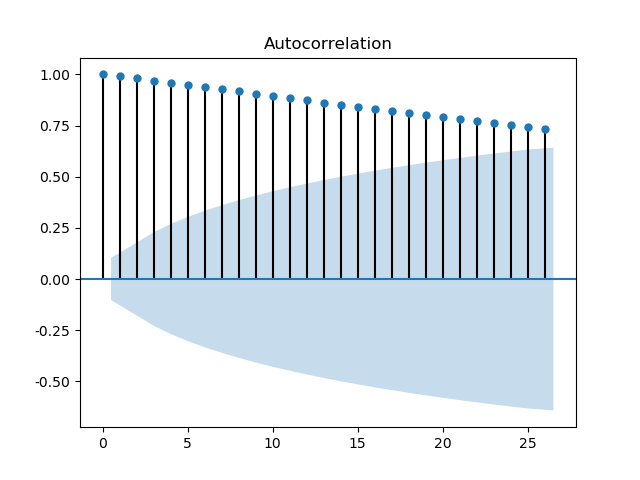
\includegraphics[width=11cm]{1.jpg}
\end{figure}
\textbf{Вывод.} При небольшом различии в количестве произведенного оружия из стали обеих компании очевидно, что число браков среди произведенных мечей из стали компании Westeros Inc. заметно больше, чем у Harpy Co. Поэтому и относительная частота появления дефекта при сотрудничестве с первым поставщиком выше.
\end{frame}

\begin{frame}{Доли сломанных мечей в i-ый месяц эксплуатации}
\begin{figure}
\centering
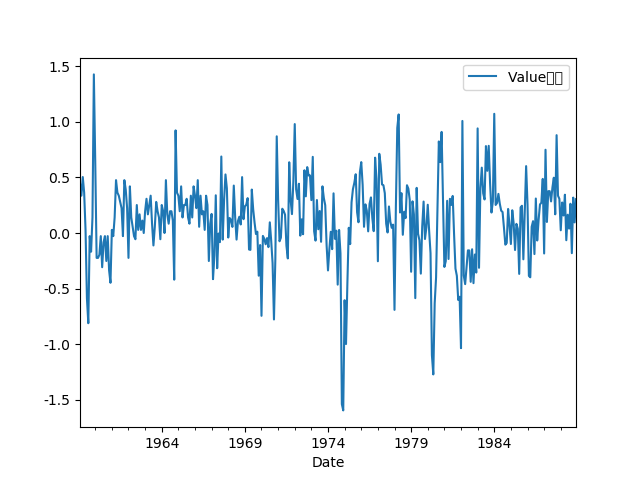
\includegraphics[width=6cm]{2.jpg}
\end{figure}
\textbf{Вывод.} Больше всего мечей из стали Westeros Inc. ломается в первый месяц эксплуатации, далее наблюдается тренд на понижение. Возможно, это связано с неоднородностью материала, поэтому брак отсеивается со временем, что может гарантировать долгую службу оставшегося оружия. Касательно компании Harpy Co: за первые три месяца после изготовления она значительно превосходит своего конкурента, так как доля сломанных мечей мала. Однако далее их число резко возрастает и мечи ломаются чаще. При этом сложно оценить последующее поведение показателей.
\end{frame}

\begin{frame}{Доли сломанных мечей на следующий месяц после производства}
\begin{figure}
\centering
\includegraphics[width=11cm]{3.jpg}
\end{figure}
\end{frame}

\begin{frame}{Доли сломанных мечей на следующий месяц после производства}
Мы понимаем, что на качество исходного материала могли повлиять различные факторы. Например, поставщик сменил источник, из которого он добывал сталь. Такие изменения могли привести к резкому ухудшению или улучшению исходной продукции. 
\newline\textbf{Вывод.} Из построенной гистограммы видно, что никаких аномалий за рассматриваемый срок не было, поэтому качество поставляемой стали обеими компаниями не изменялось.
\end{frame}

\begin{frame}{Доли сломанных мечей на i-ый месяц эксплуатации}
\begin{figure}
\centering
\includegraphics[width=11cm]{4.jpg}
\end{figure}
\end{frame}

\begin{frame}{Доли сломанных мечей на i-ый месяц эксплуатации}
\textbf{Вывод.} Заказчику важно, чтобы каждый месяц было как можно больше целых мечей, что является эквивалентным минимальной доли сломанных за месяц. Если заключить долгосрочный контракт с Harpy Co, то первые 3 месяца целых мечей при одинаковом объеме производства будет больше, чем при заключении соглашения с конкурентом. Однако в дальнейшем скорость поломки оружия будет резко возрастать в отличии от мечей из стали Westeros Inc.  
\end{frame}

\begin{frame}{Вывод}
В процессе анализа мы получили спорные результаты. Если известно, что военные действия будут длиться не более 3-ёх месяцев, то однозначно выгоднее заключать контракт с Harpy Co. Но если планируется долгосрочное сражение, следует заключать договор с Westeros Inc., так как поведение стали в их случае более предсказуемо и можно заранее распланировать необходимый объем производства.  Например, изначально произвести больше мечей, со временем брак отсеется, и во время военных действий не нужно будет отвлекаться на массовое производство. 
\end{frame}

\end{document}